\section{Race condition}

Questo attacco può essere molto pericoloso in alcune situazioni, come nel caso 
di computazioni eseguite su architettura \textit{CUDA}, in cui era 
possibile estrarre informazioni sensibili durante la computazione. In ambiente 
\textit{cloud} è importante assicurarsi che ci sia un \textit{hypervisor} che 
coordina tutte le computazioni.

Una situazione del genere può accadere in società di esplorazione geologica (eni 
ad esempio) o in situazioni di sequenziazione genomica/proteica.

\section{Messaggi d'errore troppo verbosi}

A volte i messaggi di errore sono troppi verbosi e possono far inferire delle 
informazioni. Un messaggio di errore troppo verboso è solitamente il form di 
login: in alcuni servizi sono presenti messaggi come ``password scorretta'', che 
permette all'attaccante di sapere che esiste un login con quell'indirizzo 
e-mail.

\section{External Control of Path}

Normalmente quando si ha un sito web bisogna settare i diritti. Se dall'esterno 
si può lanciare un file (es. file Word) si fornisce una backdoor per un 
potenziale attaccante.

\section{Uso di software non fidato}

Il software a volte installato dall'utente non è fidato, (es. uno 
\textit{spyware} che si occupa di raccogliere informazioni a scopo pubblicitario 
o di profilazione).

Il software free è sicuro? Sì, ma solo se è \textit{open-source} e ha un po' di 
``anzianità'' (viene utilizzato da un po' di tempo).

\section{Problemi classici di sicurezza}

\begin{verbatim}
Security() {
 String contents, environment;
 String spath = "security.dat"
 File security = new File();
 if (security.open(spath) > 0) {
  contents = security.read();
  environment = security.read();
 } else
  print("Error: Security.dat not found");
}
\end{verbatim}

Questa porzione di codice contiene diversi errori:
\begin{itemize}
\item Errori troppo verbosi;
\item Il file viene salvato in chiaro;
\item Non viene chiuso il file dopo la lettura;
\item Non viene controllata la lunghezza della lettura del file.
\end{itemize}

Un altro errore è:
\begin{verbatim}
purchaseProduct() {
 password ="N23m**2d3";
 count = form.quantity; //input
 total = count * product.cost();
 Message m = new Message(name,password,product,total);
 m.myEncrypt();
 server.send(m);
}
\end{verbatim}

Ci sono errori gravi in questo pezzo di codice:
\begin{itemize}
\item Le password vengono salvate sul codice (detto anche \textit{hardcoded}):
\item Ci potrebbe essere un \textit{overflow} (es. uno \textit{shift-bit});
\item Viene usata una routine locale per eseguire la criptazione dei dati, 
mentre si dovrebbe sempre utilizzare algoritmi standard.
\end{itemize}


\paragraph*{Come evitare gli errori} Un modo per evitare questi errori è 
testare adeguatamente il software che viene scritto. Purtroppo non è possibile 
testare il programma con tutti gli input possibili, quindi è necessario 
controllare il software con una \textit{test-suite} adeguata. 
Anche il \textit{model-checking} è importante per analizzare il software.

\subsection{Esercizi}

La parte di esercizi riguardo questa sezione è disponibile in \ref{es:Controlli}

\part{Controlli di sicurezza}

Questo modulo si concentra sui controlli di sicurezza del software. Per fare ciò 
dovremo vedere il ciclo di vita del software, con un occhio alla sicurezza.
Partiremo dall'analisi dei requisiti, per andare all'analisi del rischio e per 
finire con lo sviluppo del software.
Anche l'ambiente produttivo richiede attenzione: è importante il mantenimento da 
parte di vista della sicurezza per non introdurre bug nel software.

\begin{figure}[h!]
        \begin{center}
                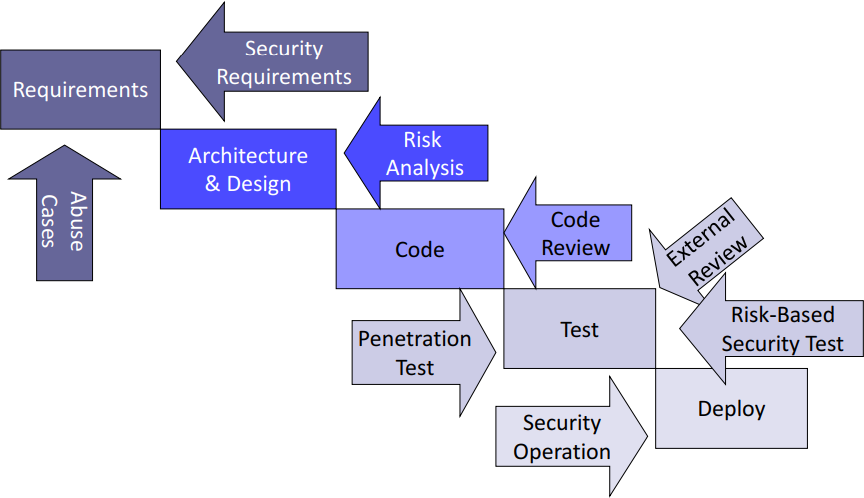
\includegraphics[width=\textwidth]{security_software_development}
        \end{center}
        \caption{La sicurezza nello sviluppo del software}
        \label{fig:security:software:development}
\end{figure}



Nell'immagine \ref{fig:security:software:development}:

\begin{enumerate*}[label=\alph*)]
	\item Abuse cases (invece di use cases) si riferiscono ai  tipici 
	casi in cui il sistema può essere flesso in chiara violazione delle
	policy di sicurezza;
	\item La Code review consiste anche nell'analisi statica;
	\item Il Test sul software è inteso come penetration test, stress test, ecc.
\end{enumerate*}






